\documentclass[11pt, openany]{book}              % Book class in 11 points
\parindent0pt  \parskip10pt             % make block paragraphs
\raggedright                            % do not right justify
\usepackage{graphicx}\usepackage{amsmath,amsfonts,amssymb,amsthm}
\usepackage{mathtools}
\usepackage{commath}
\usepackage[sc,osf]{mathpazo}

\usepackage{titlesec}

\setcounter{secnumdepth}{4}

\titleformat{\paragraph}
{\normalfont\normalsize\bfseries}{\theparagraph}{1em}{}
\titlespacing*{\paragraph}
{0pt}{3.25ex plus 1ex minus .2ex}{1.5ex plus .2ex}


% operators

\let\oldnorm\norm   % <-- Store original \norm as \oldnorm
\let\norm\undefined % <-- "Undefine" \norm
\newcommand\tab[1][1cm]{\hspace*{#1}}
\DeclarePairedDelimiter\norm{\lVert}{\rVert}
\DeclareMathOperator*{\argmax}{arg\,max}  % in your preamble
\DeclareMathOperator*{\argmin}{arg\,min}  % in your preamble
\DeclareMathOperator{\E}{\mathbb{E}}


%\graphicspath{ {./images/} }
\title{\bf Quantitative Investment Handbook}    % Supply information
\author{Xinhe Liu}              %   for the title page.
\date{2018-5-28}                           %   Use current date. 

% Note that book class by default is formatted to be printed back-to-back.
\begin{document}                        % End of preamble, start of text.
% \frontmatter                            % only in book class (roman page #s)
\maketitle                              % Print title page.
\tableofcontents                        % Print table of contents
\mainmatter                             % only in book class (arabic page #s)

\part{Financial Market and Investment Tools}

\chapter{Economics and Econometrics}

\section{Macroeconomics} 

GDP, Inflation and Unemployment:

\begin{itemize}
    \item GDP = C + I + G + X 
    \item CPI, RPI, PPI, Core CPI, Nonfarm Payroll, HICP (Europe)
    \item Philips Curve(Inflation and Unemployment)
    \item Unemployment Rate(labor force), Participation Rate(total population), Quit Rate 
    \item Unemployment: Frictional, Cyclical, Structural, Seasonal, Voluntary 
\end{itemize}


Economic indicators(manufacturing, stock prices, money supply) leading, concident and lagging indicators(employment, labor, consumer market):
\begin{itemize}
	\item Leading Indicators \\
	\begin{itemize}
    	\item PMI, Tanken Survey(Japan)
    	\item Capacity Utilisation 
    	\item Retail Sales
	\end{itemize}
	 \item Consumer Sentiment/Confidence 
\end{itemize}

Market Data Release Time Schedule:

\begin{center}
 \begin{tabular}{||c c||} 
 \hline
 Time & Market Data \\ [0.5ex] 
 \hline
 Week 1 & Employment Situation (First Friday), ISM \\ 
 Week 2 & Retail Sales, Consumer Sentiment \\ 
 Week 3 & CPI, IP \\ 
 Week 4 & Durable Goods, GDP, Consumer Sentiment(UoM final \& Conference Board) \\ 
 \hline
\end{tabular}
\end{center}

Fiscal Policy and Monetary Policy:

\begin{itemize}
	\item General Economic Goals: Full Employment, Economic Growth, Low Inflation
	\item Fiscal Policy: Government Spending and Tax Policy
    \item Monetary Policy: Open Market Operations, Discount Rate, Reserve Requirement, Federal Fund Rate(Upper Limit for Repo Rate) (In other countries: Overnight discount rate, Refi Rate, Deposit Rate, Main Lending Rate) 
    \item Interaction: Crowding Out: Higher Interest Rates may cause investment and consumption 
    \item Central bank, Taylor rule
\end{itemize}

\subsection{Business Cycle and Debt Cycle}

According to Ray Dailo's Opinion, business cycles are created by credit (borrowing). Growth = Productivity Growth + Debt Cycle Effect.  

\begin{itemize}
	\item Total output = Price $\times$ Quantity, while Price = Money + Credit
		\subitem output gap
	\item Long term debt cycle: 75 to 100 years. Short term debt cycle" 5-7 years
	\item Key indicators Inflation, deflation, tax, government spending, unemployment (Government Action)
	\item "Beautify Deleveraging": The phase total debt decreases. Needs: Spending cut, Debt Restructuring, Wealth transfer, Print Money (Government Debt increases, total debt decreases, if not carefully, lead to hyper-inflation
	\item 2-3 years depression/deleveraging and 7-10 yeas "reflation"
	\item Inventory Cycle and Business Cycle:
	\subitem \begin{enumerate}
		\item Initial Recovery: inflation still declining, fiscal stimulus, short rates low and decline, bond yields boom, stock prices rise, confidence rebound
		\item Early upswing: inflation low and growth high, short rates move up, bound yield stable and up slightly, stock trending upward, high confidence
		\item Late upswing: inflation pick up, fiscal policy restrictive, short rates rise, stock topping out, volatility could be high, confidence boom mentally
		\item Slowdown: inflation accelerate, inventory correction begins, confidence drops, short-term interest rates peking, bond yields topping out and star to decline, stock decline
		\item Recession: short rates decline, bond yields drop, stock bottoming and starting to rise
	\end{enumerate}
	\item How monetary policy works and Taylor's Rule, Kayesian Theory 
	\item Growth theory: Capital, Technology and Population, Solow Growth model, total factor productivity 
	\item Emerging market and country risk: fiscal and monetary policy, growth prospect, currency and external account (relies on the credit of foreign currency and foreign reserve), external debt and liquidity
\end{itemize}



\section{Financial Economics}
\begin{itemize}
    \item Rationality. Utility Theroy, Indifference Curve, Risk Aversion. Participants are perfect optimizers with perfect Bayesian Information
    \item Efficient Market Hypothesis : 3 Forms
    \item Market Anomalies: Fundamental Anomalies (Factor), Technical Anomalies, Calendar Anomalies, Limits to Arbitrage 
\end{itemize}

\section{Behavioral Finance}

\begin{itemize}
    \item Behavioral Finance micro: Assumes limited information, bounded rationality
    	\subitem Prospect Theory
    	\subitem Neuroeconomics
    \item Behavioral Finance macro
    	\subitem Challenge Efficient Market Hypothesis(EMH): Anomalies
    		\subsubitem Fundamental Anomalies: (eg. Value Factor, Factor Models)
    		\subsubitem Technical Anomalies (Moving Average, Support and Resistance)
    		\subsubitem Calendar Anomalies
    		\subsubitem Due to other reasons such as Limits to Arbitrage
    	\subitem Asset Pricing: Behavioral Stochastic Discount, Sentiment Risk Premium
    	\subitem Behavioral Based Portfolio Theory
    	\subitem Adaptive Market Hypothesis
    \item Behavioral Biases in investing
    	\subitem Cognitive Errors-Belief Perseverance Bias 
    		\begin{itemize}
    		\item Conservatism (Systematically review and update new information)
    		\item Confirmation Bias( Review screening criteria, promote diversification),
    		\item Representativeness Bias( Review Base-rate Neglect and Sample-size Neglect, check if forecast based solely on new data, check if treat complex and simple information equally),
    		\item Illusion of Control(excessive trading, lack of diversification, need to keep records and manage info)
    		\item Hindsight Bias(overestimate the degree of prediction, rightness of selection (manager or investment)
    		\end{itemize}
    	\subitem  Cognitive Errors-Information Processing Bias 
    		\begin{itemize}
    		\item Anchoring and Adjustment (stick to original information)
    		\item Mental Accounting( under-diversify, distinction of income and capital appreciation) Framing Bias(affects risk appetite)
    		\item Availability Bias: weight according to experience, relevance, under-diversify, affected by Ad
    		\end{itemize}
    	\subitem Emotional Bias
    		\begin{itemize}
    		\item Loss-Aversion: Disposition Effect: work together with Framing bias, Myopic loss aversion
    		\item Overconfidence: Under-diversify, Trade Excessively 
    		\item Self-Control Bias: Not save for long-term, taking too much/little risk, asset allocation imbalance - prefer income generating assets
    		\item Status Quo Bias: unknowingly maintain, work with Regret-Aversion and Endowment
    		\item Endowment: hold familiar, refuse to sell certain assets
    		\item Regret-Aversion: Herding, conservatism
    		\end{itemize}
\end{itemize}


\chapter{Basic Financial Concepts}                % Print a "chapter" heading

This chapter summarizes some basic financial concepts you should know about.



\section{Asset Management}

Asset Owners(Real Money): From conservative to active: Banks, Insurance Company, Defined Contribution Plan, Pension, Endowment/Foundations 

Hedge Funds(Fast Money)

Investment Purpose Statement(IPS): Consider Return, Risk, Time Horizon, Tax, Liquidity, Legal and Unique. 

\section{Accounting, Corporate Finance and Fundamental Analysis}

Accounting:
\begin{itemize}
    \item Balance Sheet, Income Statement, Cash flow Statement Basics
    \item EBIT = operating profit + non recurring expense - non-recurring income, EBITDA, Operating profit, normalized net income = NI + non recurring items
    \item Gross Profit, Operating profit, profit before tax, net income
    \item Gross Margin, EBIT Margin, EBIT Margin, Net Operating Margin, Net Profit Margin 
    \item Cash flow from Operations = NI + DA +- change in inventory/accounts payable, receivable, operating items
    \item CF from investing = Capital Expenditure -+ Disposal/Purchase of Assets
    \item CF from financing = -Dividend - Share buybacks + issuance of stock/bond
    \item Equity: Preferred shares, authorized shares (maximum shares the board can issue), Treasury stock, buy back book value, Free float Market capitalization = share price * ( shares outstanding - shares not traded), Small free float: little share holder control, volatile share price, high premium in M\&A 
\end{itemize}

Capital Structure:

\begin{itemize}
	\item Operating items vs financing items ( cash, financial asset/liability, equity)
	\item Working Capital = Current Assets - Current Liabilities, Operating Working Capital = Operating Assets - Operating Liabilities(exclude cash)
	\item Inventory COGS LIFO FIFO inventory turnover
	\item Payable days, receivable days, working capital cycle (payable days - inventory days + receivable days)
	\item Leverage ratios: Debt/Equity, Total Debt/EBITDA, EBITDA/inst expense	
\end{itemize}

Credit Scoring/Credit Analysis
\begin{itemize}
    \item Credit Risk = Business Risk( Country, Economic Cycle, Industry Cycle, Currencies, Commodities, trends) + Financial Risk(Cash Risk)
    \item Creditor Cashflow Statement Net Income + D/A/non-cash items = FFO( Funds from Operations), FFO +- Decrease/Increase in OWC = Operating Cash Flow, Operating Cash Flow - Capex = Free Operating Cash Flow(FOCF)\\ FOCF + Dividends = Discretionary Cash Flow, DCF +- Acquisition, Asset Disposals, Net other sources/uses of cash = pre-financing cashflow +- Increase(Decrease) in Debt, +- Net Sale/Repurchase of Shares = Inc/(Dec) in Cash/Securities
    \item Profitability \& Efficiency Ratios: EBIT/EBITDA margin, Return on Assets, Return on Invested Capital
    \item Coverage Ratios: EBITDA/interest(net interest), EBITDA/(interest + Principal Amortization), EBIT/interest or net interest
    \item Leverage Ratios: Debt/Equity, Debt/Capital, Debt/EBITDA
    \item Cash flow adequacy Ratios: FFO/Debt, FOCF/Debt, Free Cash flow/Debt, Retained Cash Flow/Debt
    \item Liquidity Ratios: maturing debt principal this year/FFO or discretionary cash flow, Quick Ratio = (Cash + Marketable Securities + Committed un-used bank credit lines)/maturing debt principal this year.
\end{itemize}

Tax:  Effective Tax Rate, Loss Harvesting and Tax-Aware investment 

Valutaion fundamentals: 

\begin{itemize}
	\item Intrinsic Value and two approaches - absolute valuation and relative valuation 
	\item Enterprise Value = Debt + Equity Value - Cash/Cash Equivalent = Net Debt Value + Equity Value
	\item Equity Value (affected by performance (operating), investing and financing (leverage)) = Price x Shares Outstanding
	\item Asset = Enterprise Value + Non-core assets(not valued by Multiples/DCF models, like cash)
	\item Free Cash Flow Calculation: EBIT - tax on EBIT (LT tax rate x EBIT) = NOPAT (net operating profit after tax )/EBIAT, Free Cash flow = NOPAT + D\&A - capex - increase in OWC + decrease in OWC - Increase in Other net operating assets + Decrease in other net operating assets -+ change in Long term tax liabilities
	\item FCFF, FCFE 
	\item Discount Rate- Weighted Average Cost of Capital (WACC) - CAPM / required rate of return, WACC = D/(D+E) cost of net debt x (1-t) + $(rf+(r_m-r_f)\times beta)\times E/(D+E)$, D is net debt
	\item Equity Market Expectaion: Gordon Growth Model
	$$ \E(R_e) = \frac{D_0(1+g)}{P_0}$$
	Grinold-Kroner Model
	$$ \E(R_e) \ \frac{D}{P} - \Delta S + i + g + \Delta PE$$
	\item EV multipliers : EV/Sales, EV/EBIT,EV/EBITDA
\end{itemize}


Fundamental Analysis, Company Analysis and Value Investing

Management/Strategic Analysis(SWOT, Five forces etc), Industry/Region/ Sector Analysis + competitor Analysis 

\section{ Real-life trading}

\begin{itemize}
    \item Shorting a Stock: achieved by a stock-loan process of broker/dealer: broker need to borrow and put colleteral, during borrow agreement, any dividend is passed (synthetically) from the borrower to the beneficial owner. Corporate actions: borrower vote as in lender's proxy. 
    \item SHOrt squeeze: Stock with high short interest trended upwards, short side cover their shorts.
    \item Naked short: short (t+2) before borrow, can borrow/buy later.
    \item Short interest thredhold: 8\% of market cap or free float.
    \item Prime-brokerage: Agency only brokerage does not own books
\end{itemize}

\chapter{Major Asset Classes and Asset Valuation Theories}
\section{Money Market}

\begin{itemize}
    \item Overnight (O/N) reference ratesL SONIA(Sterling Overnight Index Average), EONIA, SOFR - ALl has different day count convention
    \item LIBOR Rate, STIR Futures (Cash Settlement by 100 - expected interest) , IMM Dates( Exchange for interest rate and currency futures)
    \item T-bill(1,3,6,12 Month) , T-note, T-bond
    \item Commercial Paper( Issued by best quality companies)
    \item Day Count Conventions
    \item Repo Market: Repo(seller, needs cash), Reverse Repo(buyer, owns collateral for a while)
    \item Fed Funds Rate: 
    \begin{itemize}
    	\item The Upper Bound: Interest on Excess Reserves: interest rate paid by the Fed on Excess reserves held by banks at the Fed. (many money market participants are not reserve account holders so they do not have access to the IOER). 
    	\item Lower Bound: Overnight RRP: Non-reserve account holder can earn interest by entering into an overnight reserve repo(overnight RRP)- offer each day.
    \end{itemize}
\end{itemize}

\section{FX}

Basic Concepts:
\begin{itemize}
    \item FX Market is Extremely liquid (smaller bid ask spread on equity) 
    \item Market Size High to Low: USD, EUR, Cheap Currencies: JPY(safe currency), CHF, GBP, Rich(high rate) currencies: ZAR, MXN, AUD 
    \item Uncovered Interest Rate Parity and Covered Interest Rate Parity
    \item Interest Rate Forward/Futures, Non-deliverable forwards(NDF)
    \item FX Drivers: Interest rate differential, inflation rate differential, Global M\&A/Capital Flows, Technical Drivers(Indicators), Central Bank Policies, Risk Appetite
    \item Purchasing Power Parity
\end{itemize}

\section{Equity}
Sell Side Services
\begin{itemize}
    \item Traditionally, Sales and Trading Service build around research (content stream)
    \item New Model -automation: Algo-trading, Dark pools, MiFID
    \item ETF Market: Market Maker/Specialist who issue ETF Shares to investors, buy underlying stocks with ETF or money from fund and stock exchange.
    	\subitem Physical ETF: generate return from holding all, or samples of underlying shares like index funds. Kept safe by a custodian.
    	\subitem Synthetic ETF: Entering into total return swaps with counterparty issuer. 
   		\subitem ETFs fo pay dividends monthly, quarterly, half-yearly or annual. Based on funds income net of expense and distribute to share holders on the register on record date. Paid via brokerage account. 
   		\subitem Tracking error: Annual fees are deducted Reflecting daily NAVs. 
\end{itemize}



\section{Currency/Foreign Exchange}
\section{Fixed-Income}
Basic Concepts:
\begin{itemize}
    \item Day Count Convention, Dirty Price
    \item Macaulay Duration, Modified Duration, DV01, Dollar Duration, Effective Duration
    \item Maturity Effect, Coupon Effect, Yield Effect, Coupon Frequency Effect on Duration
    \item Term Structure of Yield Curve, Expectation Theory, Liquidity Preference Hypothesis, Segmented Markets/Preferred Habitat Theory. Bond Markets: < 1 y (money market) 1-3, 3-10 (bellwehter of market movements, the major contributor for “beta” in the fixed-income portfolio) 10(long end, relatively illiquid and sensitive) 
    \item long end risks: liquidity, credit( sovereign credit), inflation, growth
    \item Carry(difference between coupon-like cash-flow and funding cost) and Roll Down: Both assumes no yield curve shift
    \item yield curve trading/fly trading, steepner, flatener, positive/negative butterfly, Barbell and Bullet
    \item Inflation Linked bonds(Linkers) UK Index-Linked Gilts, French OATi, US TIPS, JGBi. Breakeven Inflation: The difference in linker yields and nominal bond yields ( linker coupon is always lower under positive inflation) 
    \item Treasury Strips, UK Gilt Strips 
\end{itemize}

Calculations
\begin{itemize}
    \item Spot yield, par yield, forward rate, Bootstrapping
\end{itemize}

\section{Commodities}

\begin{itemize}
    \item Much more volatile than other major asset classes.(volatility from both supply/demand side)
    \item Low correlation with traditional asset classes
    \item Market drivers
    \begin{itemize}
    	\item Fear: Reduced risk appetite/ fight to real assets. Geopolitics shuts down supply chains
    	\item Currencies; Gold-USD, Oil-USD
    	\item OPEC, Freak weather, earthquake
    \end{itemize}
    \item Commodity Currencies: IMF found 22 commodity currencies ( CHF-copper, AUD-Iron Ore,uranium)
    \item Stocks-to-Use Ratio, Reverse-to-Production Ratio
    \item Oil: Brent
    \item Physical Trade vs Derivatives(liquidity and leverage, low cost, less exotic)
    \item BSCOM, GSCI 
    \item Commodity Futures, Convenience Yield, Contango(normal), Backwardation(Reversed)
\end{itemize}

Calculations
\begin{itemize}
    \item Yield = Collateral Yield + Roll Yield/Cost + Spot Return
\end{itemize}

\begin{enumerate}
 \item NPV and IRR 
 \item Discounted Cash Flow Model
  \begin{itemize}
    \item Free Cashflow
    \item Required Rate of Return = Cost of Capital = Risk-adjusted discount rate : Usually from the CAPM
   \end{itemize}
 \item Valuation using Multiples - P/E, P/B 
 \end{enumerate}

\section{Derivatives}

Swap
\begin{itemize}
    \item Interest Rate Swap - fixed bond + floating bond (received swap position: long fixed bond, short floating/FRA, duration/DV01 is the difference of these two)
    \item Asset swap: Asset manager pay fixed, receive float, subject to credit risk
 \end{itemize}

Futures
\begin{itemize}
    \item long futures/ long cash = "funded beta"
     \item Used in asset-management: Tactical Asset Allocation, Beta management, Volatility Management
     \item Mark-to-market : "A martingale", variation margin changes everyday, fixed on EDSP -Exchange Delivery Settlement Price at the last day, cash settlement
     \item Open interest(\# of net short contracts) vs volume(activity)
     \item Basis and Basis Risk: divergence of futures and underlying
\end{itemize}

CDS(Derivative)
 \begin{itemize}
    \item Reference entity(borrower or obligor), reference obligation, obligations(trigger to credit event), deliverable obligations(usually pari-passu or senior in priority of payment to the reference entity), portfolio(deliverable obligations the protection buyer elects to deliver, execute accrued interest), conditions to payment(Entity party must have deliveredL Credit Event Notice, Notice to Public Info, Physical Settlement, etc)
    \item Fixed Coupon CDS: standardized (not "par spred") CDS: 100, 500bp(High Yield): T0 payment moves
    \item CDS pricing: probability of default x exposure of default x Loss Given Default  - driven by time, rates, spread
 \end{itemize}

Credit Value Adjustment(CVA)
 \begin{itemize}
    \item pricing according to credit worthness of the counter-party
    \item Volatility ~ market volatility, probability of counterparty default 
    \item Funding Value Adjustement(FVA): uncollatteralised position hedge with collateralised
    
\end{itemize}

\subsection{Option}

Credit Value Adjustment(CVA)
 \begin{itemize}
    \item Black-Scholes Model, Black's Model, Black-Scholes Equation (Heat Equation)
    \item Pricing factors and Greeks $\Delta,\Gamma, \theta, \nu$(vega), vanna, $\rho,\epsilon$ 
    \item Pricing American Option
    $$\frac{\partial V}{\partial t} + \frac{\sigma^2 S^2}{2} \frac{\partial^2 V}{\partial S^2}+ r S \frac{\partial V}{\partial S} - rV < 0 $$
    \item Option Trading Strategies
     \subitem put call parity c+pv(K) = p + S
     \subitem protective put, covered call, collar
     \subitem 1x1 spread(bull/bear), 2x1 spread, calendar spread
     \subitem risk-reversal(short p, long c)
     \subitem straddle, strangle, butterfly, iron butterfly
     \subitem volatility carry, dispersion trade
\end{itemize}



\part{Quantitative Investment Theories}

\chapter{Quantitative Portfolio Mangement}


\section{Overview and Baseline Theories}

A Basic Quant-trading System needs the following components (maybe from some teams, but need to be integrated)

\begin{enumerate}
\item Benchmark against appropriate total return index
\item Asset Allocation and Portfolio Management	framework
\item Rebalance and account for dynamic risk 
\item Risk tolerance and position sizing quantitatively (Kelly's Criterion)
\item (Optional) Market Regime Filter 
\item Cash Management and Cash-like Instruments Management
\end{enumerate}

Financial Theories involved

\begin{enumerate}
 \item Efficient Market Hypothesis (Weak, Semi-strong, Strong forms)
 \item Markowitz Portfolio Optimization
 \begin{itemize}
    \item Minimum Variance Portfolio / Tangency Portfolio 
    \item Jensen's alpha
  \end{itemize}
  \item Capital Asset Pricing Model(CAPM) Model \\
        $$ r = \beta(r_m - r_f) + r_f $$
 		$$\beta = \frac{cov(r,r_M)}{var(r_M)}$$
  \item APT(Arbitrage-Free-Pricing) Model 
 \item No-arbitrage(weak, strong) and Law-of-one-price
 \item Metrics
  \begin{itemize}
    \item Sharpe Ratio
    \item Jensen's alpha
    
        \item Required Rate of Return = Cost of Capital = Risk-adjusted discount rate : Usually from the CAPM
   \end{itemize}
 \item Valuation using Multiples - P/E, P/B 
 \end{enumerate}
 
 
\section{Portfolio Optimization}

\subsection{Problems}

\begin{itemize}
	\item goal-based approach
        \subitem describing goals, constructing sub-portfolios (selecting a module)
        \subitem Active Holding Optimization - Goal based
	 \item liability-relative
         \subitem surplus optimization
        \subitem hedging/risk-seeking portfolio
         \subitem integrated asset-liability (non-linear correlation)
\end{itemize}

\subsection{Models}

\begin{enumerate}
	\item Single Period Models: Mean-variance models, Stochastic Optimization Models
		\subitem  Mixed Integer Optimization
	\item Multi-period Models: Kelly Criterion, Dynamic Portfolio Optimization, Transaction Cost \& Taxes
		\subitem  Stochastic and Dynamic Optimization
\end{enumerate}

\subsection{Mean-variance model}

\begin{itemize}
	\item Optimization
$$ \min_{\mathbf{x}} \mathbf{x^TVx} $$
$$ \boldsymbol{ \mu^T x} \geq \bar{\mu}, x \in \chi$$
equivalent to 
$$ \max_{\mathbf{x}} \boldsymbol{ \mu^T x} $$
$$  \mathbf{x^TVx} \leq \bar{\sigma^2}, x \in \chi$$
or
$$ \max_{\mathbf{x}} \boldsymbol{ \mu^T x}  - \frac{\gamma}{2} \mathbf{x^TVx} $$
$$ x \in \chi$$

\item Two Fund Theorem

$$ \max_{\mathbf{x}} \boldsymbol{\mu^T x}  - \frac{\gamma}{2} \mathbf{x^TVx} $$
$$ \mathbf{1^Tx} = 1$$

Solution 

$$ \mathbf{x^*} = \lambda \frac{1}{\boldsymbol{1^TV^{-1}\mu}}\boldsymbol{V^{-1}\mu} + (1 - \lambda)\frac{1}{\mathbf{1^TV^{-1}1}}\mathbf{V^{-1}1}$$

$$\lambda = \frac{\boldsymbol{1^TV^{-1}\mu}}{\gamma}$$

Notice, 

\tab $\frac{1}{\mathbf{1^TV^{-1}\mu}}\boldsymbol{V^{-1}\mu}$ is the solution of $\min_{\mathbf{x}} \mathbf{x^TVx}, \mathbf{1^Tx} = 1$

\item One Fund Theorem

Add a risk-free asset into the portfolio

$$ \max_{\mathbf{x}} (\boldsymbol{\mu} - r_f\mathbf{1^T}) \mathbf{x} - \frac{\gamma}{2} \mathbf{x^TVx} $$

Solution

$$ \mathbf{x^*} = \lambda \frac{1}{\mathbf{1^TV^{-1}}(\boldsymbol{\mu} - r_f\mathbf{1^T})}\boldsymbol{V^{-1}}(\boldsymbol{\mu} - r_f \mathbf{1^T})$$

$$\lambda = \frac{\mathbf{1^TV^{-1}}(\boldsymbol{\mu} - r_f\mathbf{1^T})}{\gamma}$$

\item Characteristic Portfolio

$$\frac{1}{\boldsymbol{1^TV^{-1}a}}\boldsymbol{V^{-1}a}$$

for attribute $\mathbf{a}$

\item Common Constraints imposed on portfolio optimization would be
	\begin{itemize}
		\item Long-only
		\item Budget Constraint 
		\item Bounds on exposure to sectors
		\item Bounds on individual positions (idiosyncratic risk)
		\item Turnover constraints
	\end{itemize}
\end{itemize}

\subsubsection{Mean-variance short-comings and solutions}

Problems
\begin{itemize}
	\item Markowitz's Curse: Underperformance to market-cap weighted portfolio and concentration on assets.
	\item Estimation of mean and covariance matrix
	\item  Allocating to less liquid asset class - (no investable benchmark)
	\item Intergrality constraints: Problem becomes non-convex and difficult to solve
		\subitem e.g.Using stocks to track benchmark index - need to be solved by heuristic approach
		\begin{itemize}
			\item Forward Selection: start with one, add at a time
			\item Backward Selection: start with whole set, selecting one creating least loss
			\item Clustering approach: pick q stocks from different clusters, start with benchmark weight, optimize
			$$ \argmax _{\mathbf{x,y}} \sum_i \sum_j \rho_{ij} x_{ij}$$
			$$ \sum_j y_j = q, \sum_j x_{ij} = 1$$
			$$ x_{ij} \leq y_j $$ y is binary to indicates a stock is selected or not
		\end{itemize}
\end{itemize}

Solutions
\begin{itemize}
	\item Monte-Carlo simulation
	\item resampled mean-variance optimization
    \item add additional constriants (other than budget) - concentrated position
    \item resampled mean-variance
    \item  non-normal optimization approach
     \item Covariance matrix shrinkage estimators
      \subitem Stein's Paradox 
      $$\hat{mu} := (1-\omega) \bar{\mathbf{r}} + \omega(\mu_0 \mathbf{1}),\omega \in [0,1]$$
      \subitem Ledoit-Wolf
      $$\hat{\mathbf{V}} := \omega\hat{\mathbf{V}} + (1-\omega)\mathbf{V}_0 ,\omega \in [0,1]$$
      $\mathbf{V}_0$ is prior estimator(constant or single-factor implied cov matrix) 
     \item Black-Litterman Model (Reverse Optimization - Also less sensitive to inputs)
     $$ \mu \sim N(\mathbf{\pi}, \mathbf{Q})$$
     $$ \boldsymbol{P\mu} = q$$ (views)
     $$ \hat{\boldsymbol{\mu}} = \E[\boldsymbol{\mu} | views] = \boldsymbol{\pi} + \mathbf{QP^T}(\mathbf{PQP^T})^{-1}(\mathbf{q} - \boldsymbol{P\pi})$$
     By Solving
     $$ \min_{\boldsymbol{\mu}}(\boldsymbol{\mu} - \boldsymbol{\pi})^T \mathbf{Q}^{-1}(\boldsymbol{\mu} - \boldsymbol{\pi}) $$
	$$\boldsymbol{P\mu} = q$$
     $\pi$ is market consensus returns, $\mathbf{Q} = \tau\mathbf{V}$
     \item Robust Estimatiors
     \item  Risk budgeting vs factor based asset allocation(risk parity) to maximize diversification
     \subitem Marginal Contribution to Risk $$MRC_i = \frac{\partial \sigma_p}{\partial x_i} = \frac{\boldsymbol{Vx}_i}{\sqrt{\mathbf{x^TVx}}}$$
     \subitem Risk Contribution $$ x_i \dot MRC_i = \frac{x_i \boldsymbol{Vx}_i}{\sqrt{\mathbf{x^TVx}}} = \frac{\sigma_p}{n}$$
     \subitem Use Different Risk Measures
      \begin{itemize}	
      	\item Variance
      	\item Mean Absolute Deviation $$MAD(r) = \E( |r-\mu|)$$ $$ MAD = \sqrt{\frac{2}{\pi}} \sigma $$ under Normal
      			$$ \argmin_{\mathbf{x}} MAD(\mathbf{r^Tx})$$
      			s.t. $\mathbf{x} \in \chi$ often solve by scenario optimization
      	\item Value at Risk
      	\item CVAR (Asset Stress Loss)
      	$$ \E(Y| Y \geq VaR_{\alpha}(Y)) = min_{\gamma} (\gamma + \frac{1}{\alpha} \int_{-\infty}^{\infty} max(y - \gamma, 0) f(y) dy)$$
      \end{itemize}
\end{itemize}	

\subsection{Stochastic Optimization and Multi-Period Model}

\subsubsection{Kelly Crierion}

The Kelly Criterion is well-known among gamblers as a way to decide how much to bet when the odds are in your favor. 

The simple rule goes like this. Suppose that with probability p you will make a profit of b times what you bet, and otherwise you lose the bet. Then the optimal amount to bet is $\frac{pb−(1−p)}{b}$

\subsubsection{Dynamic Portfolio Optimization}

Some random variables value will reveal during each stage. 

\begin{itemize}
	\item Simple case. Under log utility $U(W) = log(W)$ or i.i.d. return, a myopic policy is optimization. 
\end{itemize}

Common Problems as
\begin{itemize}
	\item Mulit-stage optimization with income
	\item Portfolio optimization with trading cost
	\subitem Almgren-Chriss Model
	$$ S_k = S_{k-1} + \sigma \xi_k - g(y_k), \tilde{S_k} = S_{k-1} - h(y_k)$$
	$\xi_k$ is random shork, g and h are permanet and temporary market impact $\tilde{S}$ is captured price for trade y.
	$$Cost(\mathbf{x}) = S_0 X - \sum_{k=1}^N \tilde{S}_k y_k$$
	$$ \argmin_{\mathbf{x}} (\E(Cost(\mathbf{x}))- \lambda var( Cost(\mathbf{x})))$$
	k is trading times, $t_k = k \tau$, $\mathbf{x} = (x_0,...x_N)$ is trading trajectory, $\mathbf{y}$ is "trade list", $y_k = x_k - x_{k-1}$
	\item Sequential Decision Problem and Bellman's Optimality Principle
	\subitem Solve 
	$$ J(\mathbf{s}_0) = \argmax _{\mathbf{x_0},...,\mathbf{x_T}}[ \sum_{t=0}^N g_t(\mathbf{s}_t, \mathbf{x}_t) + g_{T+1}(\mathbf{s}_{T+1})]$$
	by solving the value-to-go of the tail problem
	$$ J(\mathbf{s}_t) = \argmax _{\mathbf{x_t}}[ g_t(\mathbf{s}_t, \mathbf{x}_t) + g_{t+1}(\mathbf{s}_{t+1})]= \argmax _{\mathbf{x_t}}[ g_t(\mathbf{s}_t, \mathbf{x}_t) + g_{t+1}(f_t(\mathbf{s}_t, \mathbf{x}_t)] $$
	f is the law of motion, which is needed
\end{itemize}

\subsubsection{Garleanu-Pedersen's Model}

Model of Dynamic Programming with predictable returns and t-costs

Problem
\begin{itemize}
	\item Minimize risk and transaction costs
	\item Trading Speed trade-off: Trade a lot: more alpha, less risk, more t-costs 
	\item ALpha (Decay) Speed: Fast and slow signals
	\item Trade-off between tax costs and diversification benefits may depend on the age.
\end{itemize}

\section{Tax Management in Portfolio Optimization}

set up

\begin{itemize}
	\item Capital gain tax depends on the holding period
	\item Tax rebate on loss
	\item Optimal tax trading: always realize loss, sometimes realize gains
\end{itemize}

\chapter{Factor Models}

\section{Factor Models}

Factor Models plays a key role in all components of asset management

\begin{itemize}
	\item Valuation and Market Expectation: CAPM, APT, alpha signals
	\item Risk Management: Risk attribution, stress test, risk modelling
	\item Portfolio Management: Smart beta, portfolio construction
	\item Performance: Performance attribution, style analysis
\end{itemize}

\subsection{Major Types of Factor Models}

\begin{itemize}
	\item Regression Model: Observable factor returns
	$$ \mathbf{X} =  \mathbf{a} +  \mathbf{BZ} +  \mathbf{U}$$ ,where $\mathbf{Z}$ is observable, estimate $\mathbf{B, a}$($\beta, \alpha$)
	$$(\mathbf{a,B}) = \argmin \E( \norm{\mathbf{a} + \mathbf{BZ} - \mathbf{X}}^2)$$
	$$ B = cov(\mathbf{X,Z}) var^{-1} (\mathbf{Z}), a = \E(\mathbf{X} - \mathbf{B}\E(\mathbf{Z}))$$
	Example: CAPM (CAPM beta can be improved by shrinking towards 1
	\item Cross-sectional Model: $\mathbf{B}$ (factor loadings) is observed. Usually use weighted list squares
	$$ \mathbf{X} =  \mathbf{a} +  \mathbf{BZ} +  \mathbf{U}$$ 
	Usually solved with Weighted Least Squares:
	$$(\mathbf{a,Z}) = \argmin \E( \norm{\mathbf{a} + \mathbf{BZ} - \mathbf{X}}^2_{\Delta^{-1}})$$
	$$ Z = (\mathbf{B}^T \mathbf{\Delta}^{-1} \mathbf{B})^{-1} \mathbf{B}^T \mathbf{\Delta}^{-1} \mathbf{X}, a = \E(\mathbf{X} - \mathbf{B}\E(\mathbf{Z}))$$
	$\mathbf{\Delta}$ is often diagonal - associated to preassumed residual sizes.
	Example: most common models, and risk models such as Aximoa and Barra $\mathbf{r} = \mathbf{Bf} + \mathbf{u}$, use time series data of r to compute time series data of f
	
	\item Principal Components Model
	$$ \mathbf{X} =  \mathbf{a} +  \mathbf{BZ} +  \mathbf{U}$$
	 $$\mathbf{Z} = [Z_1, Z_2, ..., Z_n]^T$$
	 $$ Z_i = \mathbf{e}_i^T(\mathbf{X} - \E(\mathbf{X})$$
	 $$ \mathbf{e}_i = \argmax _{\mathbf{e}} var(\mathbf{e}^T\mathbf{X})$$
	 $$\norm{\mathbf{e}}^2 = 1$$
	 $$ \mathbf{e}_k^T \mathbf{e} = 0, k = 1,...,i-1$$
	 then 
	 $$\mathbf{V} = var(\mathbf{X}) = [\mathbf{e_1}, \mathbf{e_2},...\mathbf{e_n}]
	 \begin{bmatrix} 
  				 \lambda_1^2 & & \\ 
  				  & \ddots & \\
  				 &  & \lambda_n^2
	\end{bmatrix} [\mathbf{e_1}, \mathbf{e_2},...\mathbf{e_n}]
	 $$
	 Principal Components
	 $$X_i^{PC} = \mathbf{e}_i z_i = \mathbf{e}_i \mathbf{e}_i^ T(\mathbf{X} - \E( \mathbf{X})$$
	 $$\mathbf{B}= [\mathbf{e_1}, \mathbf{e_2},...\mathbf{e_n}], \mathbf{a} = \E( \mathbf{X})$$
	 
	\item Hidden Model: Try to distinguish between systematic and idiosyncratic risk 
	$$ \mathbf{X} =  \mathbf{a} +  \mathbf{BZ} +  \mathbf{U}$$ 
	want $cov(\mathbf{Z}, \mathbf{U})$ to be 0 and $var(U) = \Delta$ diagonal,
	want $\mathbf{V} = var(\mathbf{X}) = \mathbf{B}^T var(\mathbf{Z}) \mathbf{B}^T + \mathbf{\Delta}$
	Example: the APT Model
\end{itemize}


Sometimes, factor models will be used in a multi-layer fashion (eg. decompose return first be sectors, then style factors)

\subsection{Factor portfolio}

Two common approaches

\subsubsection{Signal Portfolio Approach}

This is the traditional portfolio construction approach

\begin{enumerate}
	\item From z score form the signal score (standardization, transformation, normalization)
	\item Form the signal portfolio
	\begin{itemize}
		\item Long-short: Long equal-weight (or value-weight) portfolio with high signal and equal weight( or value-weight) portfolio with low signal
		\item Ranking: use signal to rank securities. The construct a long-short portfolio with holdings
		$$ w_i = c (rank(s_i) - \frac{\sum_i rank(s_i)}{N})$$
		\item Sorting: two-fold or k-fold version of the above high-low long-short
	\end{itemize}
	\item Use signal portfolio to get expected returns($\alpha$), covariance matrix and constraints for the optimization
\end{enumerate}

After this, finalize the rebalancing frequency, investment universe etc.

\subsubsection{Consistent Portfolio Construction Approach}

By Axioma (2011)

$$\mathbf{r} = \mathbf{Bf} + \mathbf{u} = \mathbf{B}_A\mathbf{f}_A + \mathbf{B}_F\mathbf{f}_F\mathbf{u} $$

\begin{enumerate}	
	\item Factor Mimicking Portfolios: with only exposure to one of alpha sigal/factor attributes $\mathbf{a}$
	$$ \min_{\mathbf{h}}  \mathbf{h}^T  \mathbf{V}  \mathbf{h}$$, 
	$$ \mathbf{B^T}_A \mathbf{h} = \mathbf{e}_j$$
	$$ \mathbf{B^T}_R \mathbf{h} = \mathbf{0}$$
	$$ \mathbf{h} = \frac{1}{ \mathbf{a}^T \mathbf{V} \mathbf{a}} \mathbf{{V}^{-1}a}$$
	( or can be cash neutral instead of factor neutral)
	$$ \mathbf{1}T\mathbf{h} = 0$$
	$$ \E(\mathbf{f}_A) = \E (\mathbf H^T r), var(\mathbf{f}_A) = \mathbf{H^TVH}$$
	$$ \mathbf{H} := [\mathbf{h}^1, ..., \mathbf{h}^m]$$, m factors
	\item Combine to a target portfolio
	$$ \mathbf{h^P} = \argmax_{\mathbf{h,w}} \E(\mathbf{f})^T \mathbf{w} - \frac{\gamma}{2} \mathbf{h^TVh}$$
	$$ \mathbf{h} = \mathbf{Hw}$$
	\item Find the acceptable portfolio that closest to target portfolio
	$$ \min_{\mathbf{h}} (\boldsymbol{\alpha^P})^T \mathbf{h} -  \frac{\gamma}{2} \mathbf{h^TVh}$$
	$$ \Leftrightarrow $$
	$$ \min_{\mathbf{h}} \frac{1}{2} (\mathbf{h^P} - \gamma \mathbf{h})^T V (\mathbf{h^P} - \gamma \mathbf{h})$$
	
	
\end{enumerate}

\section{Alpha}

\begin{itemize}
\item alpha is from signal and based on benchmark/factor models. For example find some signal to score stocks, then compute alpha from z-scores (neutralize for risk factors)
$$\boldsymbol{\alpha} = \mathbf{z} - (\mathbf{z^T}\mathbf{x}_B) \mathbf{\beta}$$

\item Information Coefficient(IC) : Correlation between factor score/prediction and actual outcome (realized return). IC $\geq$ 0.05 is considered good
\item Grinold and Kahn’s rule of thumb (Alpha scaling)
$$ \alpha = IC \times score \times volatility$$

Usually get covariance from risk model providers (Axioma, Bloomberg, Northfield, Barra)

\item Benchmarkmark-relative mean-variance models 

$$ \min_{\mathbf{x}} \mathbf{x^TVx} $$
$$ \boldsymbol{ \alpha^T x} \geq \bar{\alpha}, x \in \chi$$
equivalent to 
$$ \max_{\mathbf{x}} \boldsymbol{ \alpha^T x}  - \frac{\gamma}{2} \mathbf{x^TVx} $$
$$ x \in \chi$$

we get $$ \mathbf{x} = \frac{1}{\gamma} \boldsymbol{V^{-1}\alpha}$$

\item Fundamental law of active management
\subitem From above solution $$IR = \sqrt{\alpha^T\boldsymbol{V^{-1}\alpha}}$$
$$\alpha_i = IC \dot \alpha_i \dot z_i, \mathbf{V} = diag(\sigma_1^2, ..., \sigma_N^2)$$
$$IR = \sqrt{\boldsymbol{\alpha^T V^{-1}\alpha}} = IC \sqrt{N} = IC \sqrt{BR}$$
 
 \item The Fundamental Law and Transfer Coefficient
 
$$IR = \frac{\boldsymbol{\alpha^T h}}{\sqrt{\boldsymbol{h^TVh}}} = \frac{\boldsymbol{\alpha^T h}}{\sqrt{\boldsymbol{\alpha^T V^{-1}\alpha}}\sqrt{\boldsymbol{h^TVh}}} \sqrt{\boldsymbol{\alpha^T V^{-1}\alpha}}$$


\end{itemize}
\section{Smart beta and Smart Alpha}                  % Print a "section" heading

long-short STS strategy
short extension( 120/20 ) Strategy
alpha and beta separation
portable alpha 

long short equities (factor) 
convertible arbitrage

\section{Risk Premia Factors}

\subsection{Size}
\begin{itemize}
	\item Small-Minus-Big factor in equity clas
	\item No longer significant as value
	\item Structural Bias - Less information from smaller business
	\item Risk Sharing - Investor's Reluctance to invest in smaller firms
\end{itemize}


\subsection{Value}
\begin{itemize}
	\item High-Minus-Low 
	\item Behavior Bias - Rebalancing Contrarian Timing Reversals
	\begin{itemize}
			\item Over-extrapolation of past growth
			\item Delayed overreaction to price trends
			\item Discomfort with "dogs" and distress
			\item generic risk premium (1/P)
			\item rational based on distress risk, dynamic betas
		\end{itemize}
	\item Who is on the other side
	\begin{itemize}
			\item Over-extrapolation or multi-year growth
			\item Long Term overreactors( chasing returns at 3-5 yr when reversal dominate)
			\item Managers attracted to glamor stocks
			\item Investors averse to some risks in value stocks
		\end{itemize}
\end{itemize}

\subsection{Momentum}

\begin{itemize}
	\item Behavior Bias 
			\begin{itemize}
				\item Herding, Confirmation Bias, Fund Flows
				\item Under-reaction to public news
				\item over-reaction to price trends
				\item Pro-cyclical risk tolerance or risk management
				\item Disposition effect
			\end{itemize}
	 \item Who is on the other side
			\begin{itemize} 
			 \item Inattentioned, conservative, overconfident
			 \item contrarians resisting the herd
			 \item investors without stop-loss rules
			 \item those handing on the losers
			\end{itemize}
\end{itemize}
\subsection{Carry}

\begin{itemize}
	\item Behavior Bias
	\begin{itemize}
			\item Skew/Tail Preference volatility jump premia
			\item Overconfident expectations of capital losses (mkt moves) that would offset the carry trade non-profit-driven flows supporting high carry
			\item generic risk premium(1/P)
			\item liquidity needs, price pressure
	\end{itemize}
	\item Who is the other side
		\begin{itemize}
			\item tail insurance buyers, skewness lovers, crash protection seekers
			\item overconfident holders of salient macro views
			\item non-profit driven actors(central banks)
			\item Impatient/short-horizon investors, those needing immediacy in trading
		\end{itemize}
	\item Risk Sharing 
		\begin{itemize}
			\item Options: Volatility Carry, Volatility Selling
			\item Credit beta-neutral relative value trade, benefit from investor's portfolio limits(structural) providing market with insurance against credit(risk sharing)
			\item CO Curve - provide liquidity to hedgers/producers (risk sharing), higher demand from investors on near dated contracts and supply from hedgers on far dated
		\end{itemize}
	\item Structural
		\begin{itemize}
			\item Commodity Carry: Imbalance in inventory levels and subsequent hedging pressure as reflected in time spreads (eg. contango suggests selling pressure due to inventory surplus with the expectation of future price depreciation)
		\end{itemize}
	\item Koijen el el(2013) Approach
	$$ C_t = \frac{S_t - F_t}{X_t}$$ $$S_t:\text{Spot price},F_t:\text{Futures price},X_t:\text{Capital to finance futures contracts}$$
	e.g
	\subitem $$\text{Currency(CIP holds): }  \frac{S_t - F_t}{F_t} = \frac{r_t^{f,*} - r_t^f}{1+r_t^f} $$
	\subitem $$\text{Equity: } \frac{S_t - F_t}{F_t} =(\frac{ \E(D_(t+1))}{S_t} - f_t^f) \frac{S_t}{F_t}$$ $$F_t = F_t(1+r_t^f) - \E(D_{t+1})$$
	\subitem $$\text{Commodity(storage cost): } \frac{S_t - F_t}{F_t} = \frac{\delta_t - r^f_t}{1+r^f_t - \delta_t}$$ $$F_t = S_t(1+r_t^f - \delta_t)$$
	\subitem $$\text{Zero-Coupon Bond: }\frac{f_t^{(n)} - r_t^f}{1+ r_t^f} $$
	 $$S_t^{(n)} = \frac{1}{(1+y_t^{(n)})^n}, F_t^{(n)} = (1+r_t^f) S_t^{(n)} $$
	 $$C_t \approx (y_t^{(n)} - r_t^f) - D^{mod}( y_t^{(n-1)} - y_t^{(n)})$$ (slope and roll-down)
	 \subitem $$\text{Option Carry: }	 \frac{P_j(\tau -1, K, S_t, \sigma_{t,\tau-1})}{(1+r_f^t)P_j(\tau, K, S_t, \sigma_{t,\tau})} - 1 \approx \frac{-\theta_t^j + \nu_t^j(  \sigma_{t,\tau - 1} - \sigma_{t,\tau})}{(1+r_f^t)P_j(\tau, K, S_t, \sigma_{t,\tau})} - \frac{r^f_t}{1+r_t^f}$$
	 Portfolio weights
	 $$ w_i = z (rank(C_i) - \frac{N+1}{2})$$
	 z is scalar makes long-short position equals 1, N is number of stocks
	 $$ r_{t+1}^i = a^i + b_t + c C_t^i + \epsilon_{t+1}^i$$
\end{itemize}

\subsection{Betting-against Beta}

\begin{itemize}
	\item Behavior Bias
	\begin{itemize}
			\item Quality, Risk Parity
			\item Behavior Bias
			\item leverage aversion
			\item lottery seeking
			\item relative risk preferences, conventionality
			\item active managers seeking maximal bang for the (unlevered) buck
			\item Underreaction to quality
		\end{itemize}
	\item The other side
		\begin{itemize}
			\item constrained investors who avoid levering up low-risk opportunities with better SRs and instread choose concentrated high-risk exposures
			\item investors who prefer lotteries and positive skewness
			\item benchmarked managers who care more about tracking error than total portfolio risk
			\item overconfident and constrained active managers
			\item inattentioned, story-telling investors
		\end{itemize}
	\item From Margin CAPM Model(Black): Security Market Line is flatter than it should be because of margin constraints of investors
	\item Frazzini-Pedersen construction 
	   $$ \hat{\beta} = \hat{\beta}_i = \hat{\rho}_i \frac{\sigma_i}{\hat{\sigma}_M}, \beta_i = \omega + (1-\omega) \hat{\beta}_i$$
		$$ \boldsymbol{z} = rank(\boldsymbol{\beta}), \boldsymbol{\hat{z}} = \frac{\boldsymbol{1^Tz}}{n}\boldsymbol{1}$$
		$$ w_{H/L} := \frac{1}{\boldsymbol{1^T}(\boldsymbol{z}-\boldsymbol{\hat{z}})^{+/-}}(\boldsymbol{z}-\boldsymbol{\hat{z}})^{+/-} $$ 
		$$ r_{BAB,t} = \frac{1}{\beta_{L,t}}r_{L,t} -\frac{1}{\beta_{H,t}}r_{H,t}$$
		Solve
		$$ \max_{x} (\E(\mathbf{P^1} - \mathbf{P^0})^T \mathbf{x} - \frac{\gamma_i}{2} \bold{x^T\Omega x}$$
		$$ m_i (\mathbf{P^0})^T \mathbf{x} \leq W_i$$
		$$ \mathbf{x^*} = \frac{1}{\gamma}(\E(\mathbf{P^1}) - (1+\phi)\mathbf{P^0})$$
		$$ \E(r_{BAB}) = \frac{\beta_H - \beta_L}{\beta_H \beta_L}$$
	\item 
			\begin{itemize}
		 	\item Credit: Jump-to-Default
		 	\item IR Curve/CR Curve - Benediting from the average investor's leverage constraints
			\end{itemize}	
\end{itemize}

\subsection{Volatility Carry}
\begin{itemize}
	\item Risk Sharing: Comes from supply and demand imbalance of options
	\subitem Other explanations
		\begin{itemize}
		 \item sellers/buyers cannot hedge perfectly
		 \item option sellers face capital market constraints
		 \item limits to arbitrage
		 \item compensation for positive correlation with bad times and market crash
		 \item negative skewness of return
		\end{itemize}
	  \item Option supply/demand imbalances in different markets
	  \subitem
	  \begin{itemize}
	  	\item Equity: SPX(SX5E, UKX, HIS, EEM, DAX, FTSE, NKY), VIX, 10Y US Treasury Futures - downside protection in equity market
	  	\item Credit: risk management and load desks in bank are buyers. Sellers are asset managers/investors in credit market
		\item Interest Rate: buyers are banks and mortgage hedgers (protection for negative convexity in portfolio). Supply from asset manager and institutional investors looking for extra yield
		\item FX: demand from global funds to take views and hedge, supply from banks
		\item CVA Desk vs Real Trade
	  \end{itemize}
\end{itemize}

Special Considerations for volatility strategies

\begin{itemize}
	\item Volatility mark/data quality: eg. Using EEM US data to mark MXEF emerging market indices. Different trading hours, stale prices
	\item Risk Management: e.g. if hedging with futures, need funding curve mark, dividend mark, etc
	\item Hedging execution: Dealer products shorting vol(eg. CPPI, Variance Swaps, systematic selling) usually mark at close, additional Gamma position creates intraday momentum, hedging/developing strategy to monetize it. eg. For interest rate option, selection different expiries to smooth vega risk/ not fully hedge to monetize underlying mean-reversion
	\item Early exercise of American Options and corporate actions
	\item Market impact and capacity analysis
\end{itemize}

\subsection{Factor Interactions}
Value and Momentum are negatively correlated and provides diversification benefits ("Value and Momentum Everywhere" )

\subsection{Others}
\begin{itemize}
	\item Liquidity Risk Premia 
	\item Five Factor Model by Fama-French: Profitability (RMW-robustness, high OP), Investment(CMA-conservative, low INV)
	\item Seasonality: Benefiting from the market's ability to correctly estimate the seasonality of commodities (behavioral) and assume seasonality risk
	\item: COT : benefiting from the market's inability to process positioning data (behavioral) and the average investor's constraints in positioning according to such data
	\item Equity Intraday Momentum
\end{itemize}

\subsection{Practical Issues}

\begin{itemize}
	\item Universe: small stocks may have information/liquidity issues, in the same time potentially they bring more profit
	\item Bottom-Up vs Top-down approach of portfolio construction: See "Factor Portfolio" part. In practice, more constraints in the process (short transaction cost, short selling index vs short selling stocks
	\item Long-only implementation and long-short implementation
	\item Factor Sensitivity Control $\frac{\sigma_j w_j}{\sum \sigma_k w_k}$
	\item Factor Signal Processing: Mutli-window, exponential smoothing. etc
\end{itemize}
\section{Bond Factors}

common risk Premia in bonds

\begin{itemize}
	\item Carry: Term Structure of yield curve. (Compensation for bearing duration, inflation and illiquidity risk (long riskier assets))
	\item Trend: Over/underreaction
	\item Value: Yield - Inflation Expectation. (10y futures across G8, inflation consensus, as a compensation beyond expected rates path) Bond Risk Premium as compensation beyond expected rates path
	\item Volatility Selling - Demands on US IR Vol Surface are driven by different factors (expiry, tenors
	\item "Betting Against Beta" - DVO1 neutral steepener in credit CDS/Itrixx index(high beta is longer dated assets)
	\item Credit Market : beta and spread has "regime dependency" for term-structure carry. "Squeeze Sensitivity" and "Sensitivity to constituents" to 
\end{itemize}

Some bond specific risk-premia study

\begin{itemize}
	\item Fama-Bliss(1987) and Cochrane-Piazzesi(2005) on excess log return and forward spread
		$$rx_{t+1}^{(n)} = \alpha + \beta (f_t^{(n)} - y_t^{(1)}) + \varepsilon_{t+1}^n$$
	\item Ludvingson-Ng (2009) form factor of macroeconomic variables
	$$rx_{t+1}^{(n)} = \boldsymbol{\alpha^TF_t} + \boldsymbol{\beta^T Z_t} +\varepsilon_{t+1}$$
\end{itemize}


\section{Market Anomalies}

\subsection{Behavioral Finance}

Behavioral Finance Theories Includes Prospect Theory( People suffice rather than optimize, the utility curve is concave at the gain part and convex at the loss part(loss aversion). Bounded Rationality and 
Behavioral Market Anomalies/bias

\begin{enumerate}
 \item loss aversion(herding)
 \item illusion of control(TAA) 
 \item Mental accounting(goal),
 \item availability bias(familiarity, home-bias)
 \item recency bias(tactical shifts)
 \item framing(risk-return presented in a different way)
\end{enumerate}


other: liquidity risk premia
\begin{enumerate}
 \item Risk Management and Hedging 
 \item Leverage 
 \item Correlation
 \item Strategy replacements, leverage rebalancing and rebalancing frequency, leverage reset
\end{enumerate}


other: liquidity risk premia
\begin{enumerate}
 \item Risk Management and Hedging 
 \item Leverage 
 \item Correlation
 \item Strategy replacements, leverage rebalancing and rebalancing frequency, leverage reset
\end{enumerate}

\chapter{Statistical Arbitrage}

\section{mean-reversion}

intraday mean-reversion

hedge fund strategies

  merger/risk arbitrage

   fixed income arbitrage
       swap spread arbitrage
       yield-curve spread arbitrage
      mortgage spread arbitrage ( on prepayment rates)
      capital structure/credit arbitrage 
      volatility trading (interest cap vol) arbitrage

\chapter{Quantitative Trading Strategies}


\section{Strategy Toolbox List}

\begin{itemize}
	\item Signal
		\subitem Multi-signal mix: Multi-window, multi-signal
		\subitem Signal Smoothing:
			\subsubitem Exponential Decay, half-life length
	\item Weighting and Rebalancing Methods
		\subitem Strategy Groups
		\subitem e.g.
		\begin{itemize}
			\item Recovery: For volatility carry strategies, drawdown recovers fast -Using tail risk measure(Asset Stress Loss, CVar)/Long-term Based Fixed Weight is more appropriate. For trend strategies, positive weight and negative weight changes fast, so use parity when put into top level. Inside the strategy group, use weight smoothing
			\item Signal Speed: For time-series momentum strategies, correlations signals varies a a lot - using Risk Parity (ignore the correlations)/max trend exposure with volatility control
			\item For equities, constraints such on single stocks, regions, sectors, and tracking errors vs benchmarks need to be imposed as model insurance/risk controller.
			\item Additional risk-level control on beta(bond/equity), control sensitivities to certain risk factor (eg. Size and Value have high sensitivities to equity benchmarks in a cross-asset portfolio)
		\end{itemize}
	\item Risk
		\subitem Portfolio Volatility Control, Sub Portfolio Volatility Control 
		\subitem Correlation
		\subitem Leverage Control
		\subitem Volatility Target
		\subitem Idiosyncratic Risk 
	\item 
\end{itemize}

Special Concerns on the tradability/capacity of the strategy

\begin{itemize}
	\item Trading Cost and Market Impact : empirical analysis, trading cost models(quadratic impact) and rebalance frequency control
	\item Tax, Tax-aware investing
		\subitem Different rules applied to ordinary income, capital gains, capital losses. There are differences in the tax rates for long-term vs short capital gains. Wash-sale restrictions.
\end{itemize}


\section{Equity}
\section{Volatility and Dispersion Trades}
	\subsection{Volatility Models and Time-Series Models}
	
\section{fixed income + macro}
\section{fixed income derivatives}

MBS Convexity Trade

    1. real estate-direct vs indirect environment  
    2. benchmarks of real estate
    3. other alternative, commodity to hedge

\section{credit}
\section{commodities} 
\section{Cross Asset}

\begin{enumerate}
 \item Cross-Asset Risk Premia
 \item Cross-Asset Trend
\end{enumerate}


\chapter{Quant Strategies and Long-short Strategies}

Stat Arb (typically high volume), Merger Arb, Relative Value, IntraCap Pairs 
 

\part{Quantitative Modeling and Strategies Implementation}

\chapter{Strategy Development Overview}

Typically, need the sub functions/sub teams including:

\begin{enumerate}
 \item Data Curator: Data collection, cleaning, indexing, storing, adjusting and delivering 
 \item Feature Engineering and Analytics: Data Mining, Signal Extraction and Processing using information theory, Data visualization, labeling, filtering, classifiers building - try to extract features
 \item Strategies Research: Make sense of features, market observation, instrument knowledge and try to formulate general theory/intuition that explains market mechanics. Submit code to the backtesting team
 \item Backtesting: Statistical, Stochastic, Econometric tests of strategies/portfolios
 \item Deployment: Rely heavily on computing, process schedulers, automation servers, vectorization, multithreading, multiprocessing, Big Data, Machine Learning on Big Data and High-performance computing 
\end{enumerate}

Back office and Risk Management (See Risk Management chapter)

\begin{enumerate}
 \item Portfolio Aggregation
 \item Portfolio Evaluation
 \item Performance/Risk Attribution
\end{enumerate}

Also, teams should also maintain and select current strategies, typically, a strategy experiences Embargo, Paper Trading, Real-money trading, Re-allocation and Decommission.

Some Major Challenges:

\begin{enumerate}
 \item Traditional Portfolio Mangers work in silos and make decisions alone. While quant investing need to cut-down the decision making process to small research projects and run as a strategy factor
 \item Combine "black-box" PM views/market intuition with quant research results from data/math. 
 \item Combine machine learning algorithm with existing traditional strategies. 	
 \item "Backtest overfitting": Without limitation on number of trials, Sharpe ratio in back test could be very high. 
\end{enumerate}


\chapter{Financial Data Modeling}


"Garbage-in, Garbage-out". Data is the most important element. Common pitfalls as

\begin{itemize}
	\item Surviorship bias and failure to ensure non-anticipative trading
	\item Bid and Ask Spreads
	\item Transaction costs and liquidity
	\item Paper Statistical validation (backtesting set up and validation, statistical test on back-test result is a big topic)
\end{itemize}

can typically happen. 

\section{Financial Data Structure}

Basic Assumptions: Most time should check implicit assumptions

\begin{itemize}
\item Equities $log(\frac{V_{t+1}}{V_t}$ i.i.d. Liquidity varies a lot. Benchmark indices can be misleading: eg. DJIA is priced-weighted. S\&P 500 leans towards large market cap companies and not include \textbf{dividend reinvestment} (S\&P Total Return Index include)
\item Fixed Income $Y_t(\tau) = -\frac{1}{\tau} log(V_t(t+\tau))$ i.i.d shock on interest rate (bond yield)
\item Risk drivers/factors $\mathbf{X}_t = [X_{1,t}...X_{\bar{d},t}]$ homogeneous in time, and determines the joint PnL of instruments

\end{itemize}

Data Problems
\begin{itemize}
 \item Financial Data, especially economic data can be series lagged. (important data can be officially reported/audited with a quarter lag, IMF reports some country data with 2 years lag)
 \item Data Measurement errors and biases: transcription errors, survivorship bias(*), Appraisal Data (Smoothed data, which seriously influences volatility estimation, volatility factor is needed)
 \item Sampling's interaction with market regime and non-stationarity
 \item return measured less than a year includes implicit extrapolation
 \item illiquid and infrequent priced assets may be priced with
 	\subitem Matrix pricing (common in bond market)
 	\subitem Consensus/Expert Data
 	\subitem Appraisal Data: without public information, risks is underestimated 
 \item Bonds: Recall, Termination (Aging), Exchanged
 \item Stock: Corporate Actions (Splits, Reverse Splits, Voting Rights, etc)
 \item Futures and Options: Termination and Rolling
 \item Currencies: Not Traded in centralized order book 
 \item Different data collection principles and definitions, error rates in collection, change in calculation formula (eg. CPI, rescale of index), data re-scale ("rebase" of economic data)
 \item Benchmark formormulation methods, liquidity, investability,
\end{itemize}

Signals

\begin{itemize}
 \item Quote Offers canceling/replacing with sell orders 0 potnetial sell off information
 \item Limit Orders vs Market Orders 
\end{itemize}

\section{Financial Data Sampling}

\subsection{Data Sampling Methods}

\subsection{Data Sampling Weights}

\section{Time-series Data Modeling}

\section{Data Labeling in Strategy Research}

\section{Estimators}

Distinguish between
\begin{itemize}
	\item Sample Estimator
	\item Shrinkage Estimator
	\item Factor Models(imposed factor structures/PCA Structures)
\end{itemize}


\chapter{ Trading System }



\section{ Strategy Development Pipeline(Single/Linear Strategy) }
\subsection{Basic Architecture/System}
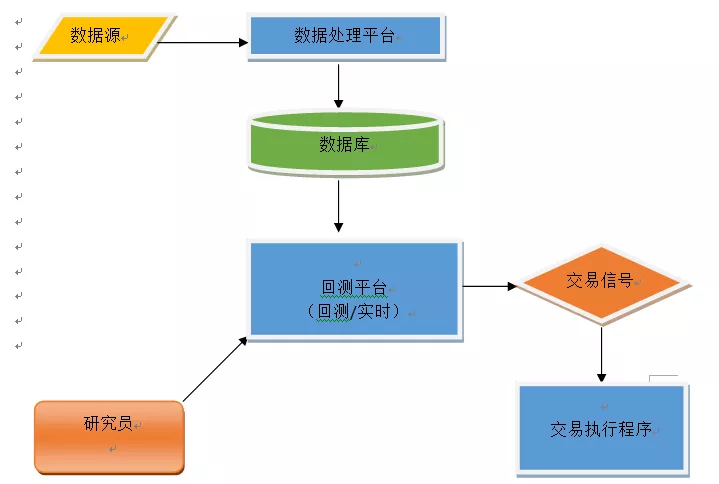
\includegraphics[scale=0.5]{1.JPG}
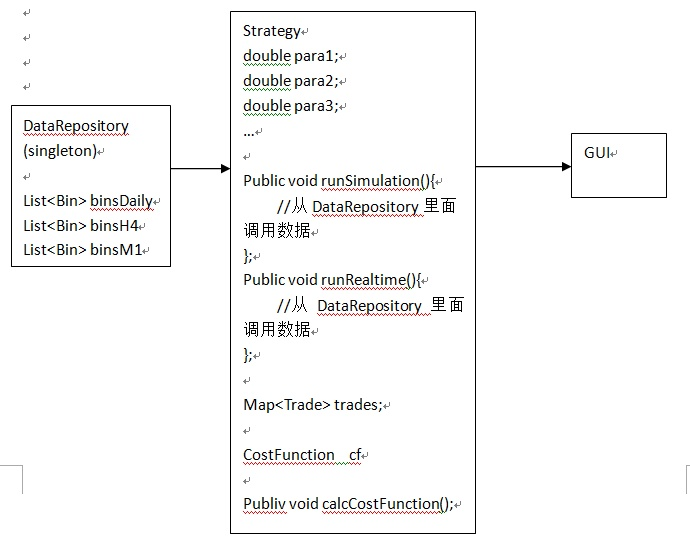
\includegraphics[scale=0.5]{2.JPG}
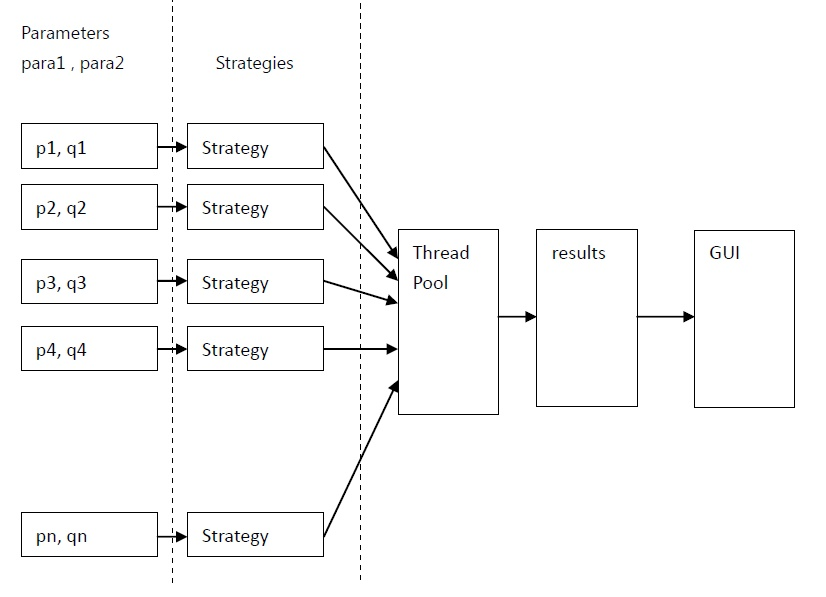
\includegraphics[scale=0.5]{3.JPG}
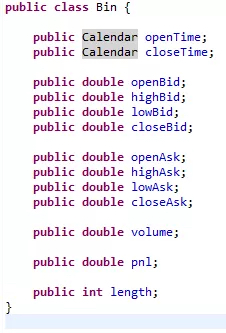
\includegraphics[scale=0.5]{4.JPG}
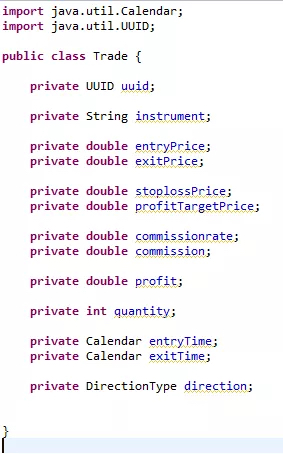
\includegraphics[scale=0.5]{5.JPG}
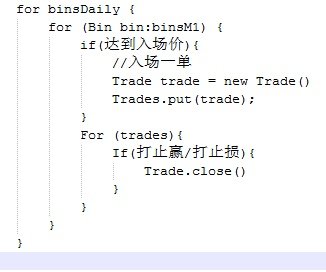
\includegraphics[scale=0.5]{6.JPG}


Historical Data is a singleton. All Market Data (eg. a candle stick ) should be organized to feed the researcher to program strategies on the backtester (eg. like quantopian). All back-testing should be parallized (ideally on GPU) to display parameter-profit relationship. (heatmap, stock charts, etc ) Ideally the optimization process could be visualized (like Tensorflow) 

All like a research facility feedback cycle. 

Key Details: API Design, Module Separation etc. 
\subsection{Data}

Key is a real-time listener. Technical Considerations: KDB, Hadoop and HDFI(?), SQL Like, Mongo Db to store Archive Data. Market Data Providers consideration buying from Wind, BBG, Reuters, Etc. \\

teams: platform operation engineer, analytics builder, strategy control/management and risk management, data team, execution team, researcher team ( 3 x tech )\\

data licensing and data quality insurance \\

data base, text file archive, big data issue\\

cheap data: brokerage: interative brokers.

\subsection{Backtester/Simulator}

Key Components

*Send Singal to Quoting/Trading/Exection Tool(Real Time)
*Market Data Objects (eg. loop for every time bins)
*stop loss/risk control system integration
*parameter-backtest profit/statistics result: optimization and loss function set function to tune the parameters
*multi-thread: Java backter (Java thread pool*)
*human selection of parameters: parameter table and visualization

\subsection{Trade Record and Money Management}

record every trade, summarize execution shortfall, statistical trends and information (shortcomings of strategy executions) and market information ( learning material) build statistics and storage

More: order book and trade book level data handling

\subsection{Analytics}

\subsubsection{ Strategy Management }, Sharpe Anslysis, Holding Period, Slippage visualization to better assistant strategic allocation

\subsubsection{Execution Analysis and Cost}

quantitative trading/systematic trading strategies:
* equity long/short

\subsection{Research Team}
Key problems:
* Optimization and Combination of Sub-Strategies (Eg. factors)
* Market Regime Change Detection(problem not solved): Distinguish between trend and oscillation market
* market supply/demand imbalance analysis (risk-premia) 
* volatility trading, dispersion trading - 2nd and 3rd degree trading, (vol model, vol clustering effect, vol leverage effect)
* hedging/overlay strategy research: hedging cost and hedging risk management, how to adjust hedge according to market condition.
* common ideas: market imbalance, mean-reversion, autocorrelation patterns etc (find patterns and trade) - based on statistics.  Risk factors, implied arbitrage - based on math. 

\subsubsection{Parameter Optmization and Control}

Rely on GUI - parameter distribution and selection
optmization methdologies from machine learning ( see optimization chapter)
robustness anslysis and out-of sample test ** ( random cut the universe of rolling window on selection period )

\subsubsection{Signal Indicator Design}

For example, based on fundemental ratio and technical indicators - design a formula. And check the level of prediction power (if any)

1.seeking stationarity: find a stationary time series
	use difference, integration, and normalize with volatility 
2.find signal level, plot cumulative back-test return against different signal level (use own quotes, and use signal level to filter quotes)
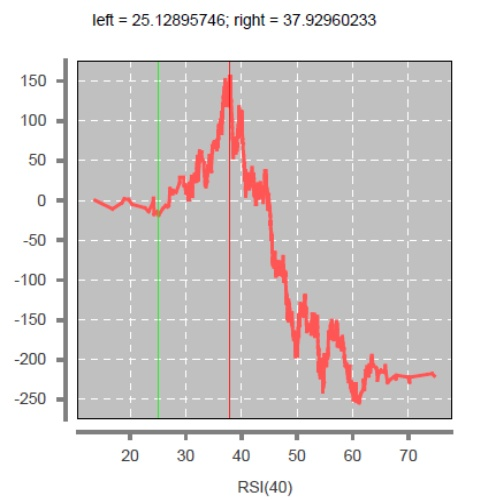
\includegraphics[scale=0.5]{7.JPG}
3.Check stability of customized indicators 
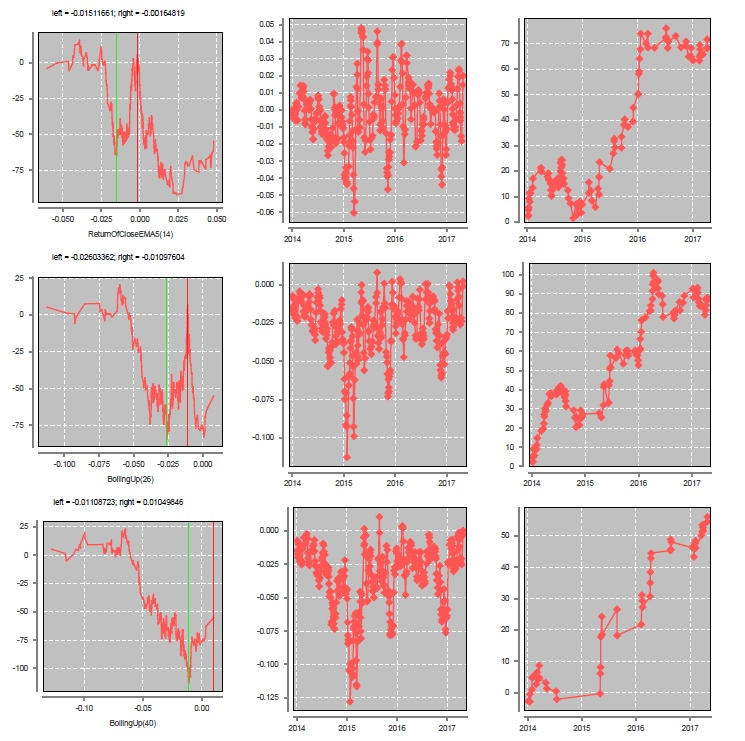
\includegraphics[scale=0.5]{8.JPG}
4. check overfitting and type-II error in all settings, apply noise filtering if possible 
5. design a interface to input indicator(math formula parser to read string) and visualize information using GUI.(HTML/XML Render)
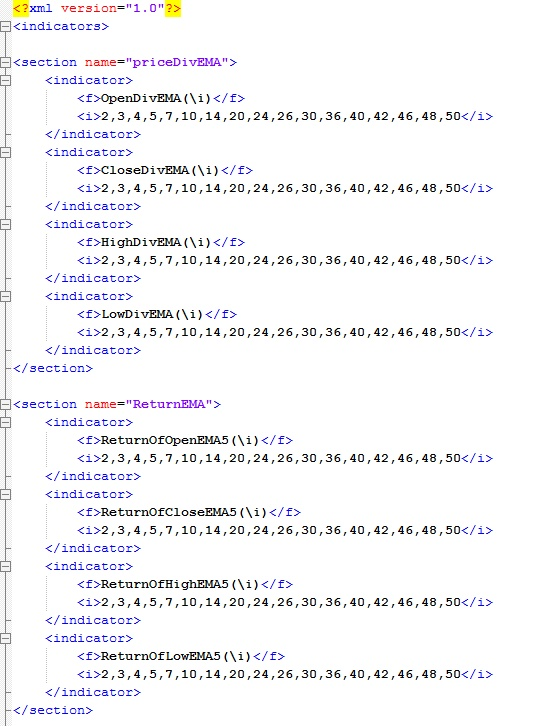
\includegraphics[scale=0.5]{9.JPG}
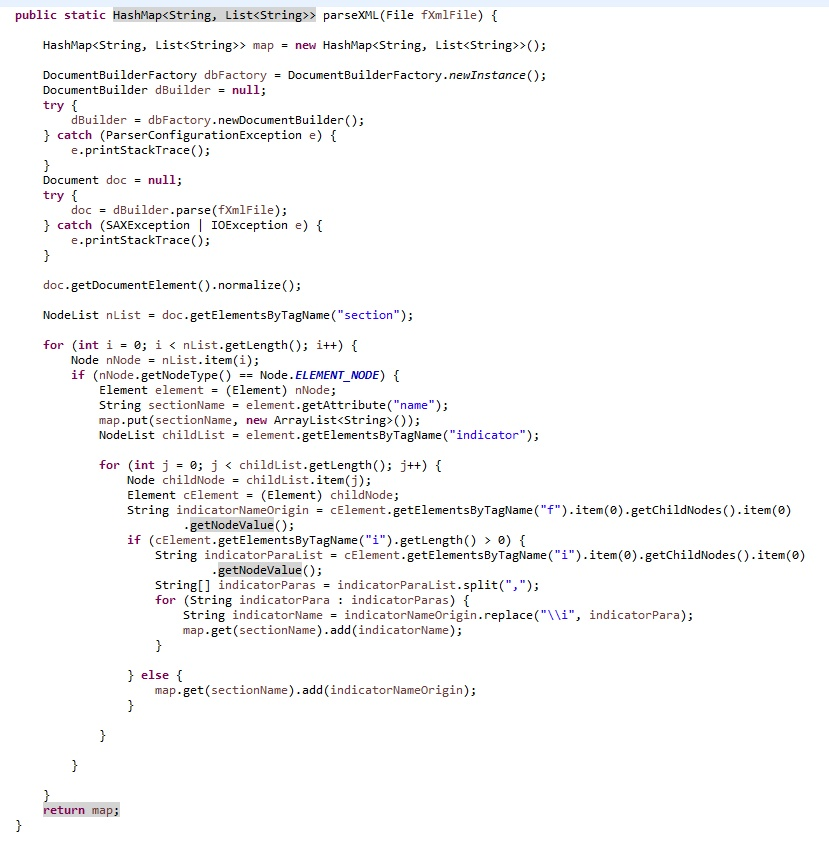
\includegraphics[scale=0.5]{10.JPG}
6. aggregate all indicators( eg. macd, ead ). Aggregate all strategies using optimization framework or selection framework to gain statistical alpha
7. indicator effectiveness test
1. test correlation - the correlation between indicator and profit vs. the correlation between correlation and white noise(hypothesis test) * use spearman correlation rather than pearson correlation* 
2. Use Monte Carlo Simulation to do permutation test of effectiveness of indicator
3. Very very hard - detect sensentivity to market regime change(osicallation and trend) and identify market regime change. 

\subsubsection{Integration of single indicators and portfolio theory}

Form indicator as factors: standardization to mean-0, normal/t-distributed scores. Select powerful ones (ones that passed the permutation test). Optimize to maximize holdings exposure to factor with risk penalty. The key is still feature engineering.

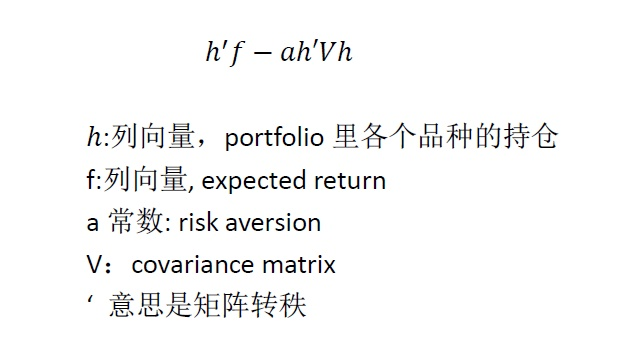
\includegraphics[scale=0.5]{11.JPG}

For Covariance, See section "covariance matrix".  



\subsubsection{Strategy Risk Management and Money management}

small stop loss, big stop gain level on reversion strategies.bigger stop loss, smaller stop gains on volatile markets - based on experience, market analysis.

Choose symmeteric/non-symmetric risk control based on market belief

Hedging and Market Exposture Management - Volatility Control and Automatic de-leveraging. 

together with cost consdieration. 

\section{Backtesting}

\begin{enumerate}
 \item Surviorship-bias
 \item Look ahead-bias
 \item In-sample bias
\end{enumerate}

\chapter{Portfolio Risk Management}

\section{Key Questions}

\begin{itemize}
\item Position Sizing: How much to bet per desired asset?
\item Vol, Skew and Kurtosis - The historical distribution of portfolio returns
\item Non-stationarity of Returns: Regime Filtering, Back Testing Results
\item Counter-party Risk
\item Operation Risk (Trading Infra fails)
\end{itemize}

\section{Derivatives and Hedging Strategies}


Sell Side Risk

Coherent  Risk measure

monotonicity

subadditivity

positive homogeneity

translation invariance



liquidity risk


funding liduitdity
market liquidity ( brokerage fees, execution price compared to mid-point, impact of transaction in the market price, the speed of transaction execution)


evidence that liquidity good: stable quoted bid-ask spread, order book depth deep, falling realized bid-ask spread, 
evidence for bad liquidity: large trades have more market impact, average trade size fall, increased bifurcation in the corporate bond market( different liquidity preferring on-the-run)


influncers

regulators( e.g. leverage, Volker Rule)

Central bank
  bank funding channel
  market functioning channel
 risk appetite channel

liquidity measures
bid-ask spread
effective spread
Roll’s price reversal 
Corwin and Schultz high-low spread 
price impact
turnover
Amihud’s measure
Markit’s liquidity score
Dealer count
Quote depth
Imputed round-trip cost






tightness: cost of a round-trip transaction
market depth: how much moved by a large order
resiliency : length of time for which a lumpy order moves the market away from the equilibrium price
adverse price impact
slippage( the amount of deterioration in the market price induced by the amount of time it takes to get a trade done)  


model validation(quantitative)

validation of inputs and parameters(assumptions)
model replication
benchmarking and hypothetical portfolio testing (with another strategy)
backtesting
profit and loss distribution
stress testing\

2. risk management
    1. Var - historical, analytical, MC good and bad
    2. credit risk exposure (pv only swap has)
3. derivatives  
    1. futures, hedge, synthetic equity/cash, pre-investing
    2. options
        1. spread-bull bear, butterfly   
        2. straddle, collar, box spread( bull, bear spread- risk free rate)
        3. interest rate swap - leveraged floating-rate notes, inverse floater; currency swap
        4. swaption - payer, receiver - use receiver to add/remove callable bond features 


1. fixed income
    1. duration matching 
        1. requirements
        2. vs cashflow matching(tenor offer), contingent immunization, horizon matching
    2. index and challenges 
        1. index vs mutual fund,ETF, synthetic strategies(total return swap, less cash but counterparyt risk )
    3. yield curve strategies
        1. laddered, bullet, barbell vs level slope curvature
        2. barbell vs bullet, condor and butterfly long short at level change, slope change, curvature change, yield volatility change performance and strategy (wing and body)
    4. high yield and credit stprad
        1. IGB HYB : credit risk, credit migration risk, interest rate risk, liquidity risk
        2. access liquidity risk and tail risk 
        3. emerging market difference 


\section{FX risk management}
    1. currency management 
        1. forward price (long/short base currency) 
        2. options- risk reversal, put spread, seagull spread
    2. index and benchmark
        1. capitalization-weighted, price-weighted, equal-weighted index, fundamental-weighted indexes 




\chapter{Monitoring and Performance Evaluation}

\section{Monitoring}
    1. rebalancing corridor width
    2. CPPI/ swaption etc

\section{Performance Analysis}

\begin{enumerate}
 \item Performance Measurement
 \subitem Measure returns: Time-weighted(TWRR) or money-weighted (MWRR)
 \item Performance Attribution
 \subitem Key is benchmark
 \item Performance Appraisal 
 \subitem Different Performance Measures
\end{enumerate}


\subsection{Performance Attribution and Style Analysis} 

Key to do performance attribution and portfolio risk management is the selection of benchmarks (ideally liquid, investable, and reflects style). Common ones like indices, manager's universe, factor model or customized benchmark can be tested by

\begin{itemize}
 \item Minimal systematic bias: (historical beta of portfolio of benchmark should be close to 1, correlation between P-B and B-M should be zero
 \item Tracking Error should be minimal
 \item Exposure to systematic risks should be similar to the portfolio
 \item Coverage (percent of market value of portfolio) should be maximal
 \item Turn over should not be excessive
 \item Active positions should be measurable and positive
 \end{itemize} 

Performance Attribution

\begin{itemize}	

 \item Macro Performance Attribution : From fund sponsor's perspective. 
 	\subitem Usually from asset class perspective: Policy Allocation + benchmark asset return + fund returns, variations, cash flows
 \item Micro Performance Attribution: To stock/asset level or to factor level (see: style analysis).
 e.g.
 $$r_v = \sum_j(w_{Pj} - w_{Bj})(r_{Bj}- r_B) + \sum _j(w_{Pj} - w_{Bj})(r_{Pj} - r_{Bj}) + \sum_j w_B (r_{Pj} - r_{Bj}) $$
 \item Style Analysis
 	$$r_p(t) = \sum w_i f_i(t) + u_p(t)$$
 	Solve quadratic optimization
 	$$\argmin var(u_p(t))$$
 	$$w_i \geq 0, \sum w_i = 1$$
 	(notice, not minimize squared error, use $t-T$ period to estimate $w_i$, then get the selection return(specific risk) \\
  \item Variations include
  
    \begin{itemize}
  	\item weight change over time, the will cause the solution to be undetermined, need to discourage large movements by regularization. 
  	\item factors usage: 
  	\subitem  fundamental factor model 
  		\subsubitem sector factor: from return to get exposure
  		\subsubitem style factor: from exposure (factor loading/factor scores) to get return. (See Factor Models)
  	\subitem macroeconomic factor models(economic factors as GDP, rates)
  	\subitem statistical factor models(PCA, Asymptotic PCAs and time varying factors) 
  \end{itemize} 
  
  \item Then decompose the risk with factors: the risk of k-th exposure weighted factor: $$\sqrt{\frac{1}{T}\sum_{l=1}^T (w_k f_k(l) - \overline{w_k f_k})^2}$$
  \item Bond portfolio performance Attribution: Same spirit but more complicated than equity portfolio: Need to separate 
  	\subitem External Interest Rate Enviroment
  	  	\subsubitem returns on default free bonds with no forward rate change
  		\subsubitem return due to the change of forward curves
  	\subitem Management Process
  		\subsubitem Interest Rate Management Effect: treat as if default free bonds
  		\subsubitem Sector Quality Effect: sector and quality group
  		\subsubitem Security Selection: within group selection
  		\subsubitem Trading Activity: residual
\end{itemize}


  
\subsection{Measure Performance}

The key purpose is to collect data and do statistical tests on alpha. 

Common Performance Measures

\begin{itemize}
 \item Jensen's Alpha (expost $E(r_p) - E(r_b)$
 $$ r_p(t) = \alpha_p + \beta_P r_B(t) + \epsilon_p(t) $$
 t-test on $\frac{\alpha_P}{SE_{\alpha_p}}$ usually use 2 as a thredhold \\
 Rule of Thumb:
 $$IR = \frac{t-stat}{\sqrt{T}}$$
 Can be used with a single benchmark, sector or style multi-factor models
 \item Ratio Measures
	\subitem Total Risk: Sharpe, M2 Measure
	\subitem Systematic Risk: Treynor Ratio
	\subitem Information Ratio: $$ \frac{r_A - r_B}{\sigma_{A/B}}$$
\end{itemize}
  


\chapter{Alternative Data and General Machine Learning}

\chapter{E-trading and Execution}

Program Trading: Trading a group of instruments, typically cash equities, as single unit (Portfolio Trading or Basket Trading) Commissions from 3bps to 15 bps (2018). Used by active funds, arbitragers (derivatives to cash (eg. Treasury and Treasury Futures)etc)

Hedge Funds use it as part of Stat Arb (typically high volume), Merger Arb, Relative Value, IntraCap Pairs


Execution, Market Impact, VWAP 


\begin{thebibliography}{999}

\bibitem{lamport94}
  Marcos Lopez De Pardo, 
  \emph{Advances in Financial Machine Learning}.
  Wiley,
  1st Edition,
  2018

\end{thebibliography}
 
\end{document}                          % The required last line 